%cSpell:ignore Erol,Sezgin,fancyhdr, hheadheighti,hheadsepi,hfootheighti,graphicx, hfootskipi, Gavrilita, Mihail, AMOO, totalheight, keepaspectratio,UML's, kata, codewars, OOAD, COFFE,ERLANG,caml, kotlin,haskel, ruby, superclass, 
\documentclass[12pt]{article}
%\usepackage[english]{babel}
%actually it works without this package//// cuz it is in english by default... it might be useful //// but not here
% \usepackage{natbib}
% \usepackage{biblatex}

% \usepackage[backend=biber]{biblatex}

%\usepackage{url}
%idk what for it is here, it is not what it seems to be, fuck it
%%\usepackage[document]{ragged2e} 
%%to justify
% i dont use it anymore
\usepackage[utf8]{inputenc}
%%%\usepackage{amsmath}
%%useless for this report... it's for math stuff
\usepackage{graphicx}
%This package enables the user to the importation of graphics into a .tex file and, apart from the usual sizing and rotational facilities, also enables the user to crop or trim an image as desired (e.g., to get rid of surrounding blank margins). The graphicx package is useful if you need to use only a part of a complete image. 
\graphicspath{{images/}}
%% includes pics inside image folder
\usepackage{parskip}
%%this shit . In the document body, don't use \parskip but a blank line to separate paragraphs.there's normally no need to add manual line breaks (\\) in the text.

\usepackage{vmargin}
%%LaTeX package which introduces paper sizes and provides macros for setting document margins. 
\usepackage{enumerate} 
%enumeration of elements  
\usepackage{caption}
%%this is for figures
\usepackage{float}
%% to position exactly the figure 
\usepackage{fancyhdr}
%%To customize the footer and header in your document first import the package fancyhdr with 
% \addbibresource{lab4.bib}
% \bibliography{my_bibliography.bib} 
\PassOptionsToPackage{hyphens}{url}\usepackage{hyperref}
\hypersetup{
    colorlinks=true,
    linkcolor=blue,
    filecolor=magenta,      
    urlcolor=cyan,
}

\renewcommand{\theenumii}{\arabic{enumii}}
\setmarginsrb{3 cm}{2.5 cm}{3 cm}{2.5 cm}{1 cm}{1.5 cm}{1 cm}{1.5 cm}
%%\setmarginsrb{hleftmargini}{htopmargini}{hrightmargini}{hbottommargini}% {hheadheighti}{hheadsepi}{hfootheighti}{hfootskipi
\title{PPE Laboratory 4}								
\author{Sezgin E}							
\makeatletter
%%The \makeatletter command temporarily defines »@« as a normal character to enable changes to internal LaTeX macros outside packages (STY) or classes (CLS).
\let\thetitle\@title
%%\let allows you to copy the content of a command into a new command.
\let\theauthor\@author
%%Thus \let\foo\bar defines \foo to have the value that \bar had at the point of definition.
\makeatother
% With \makeatother this process is reversed and the »@« is set to its original character category (other). The »@« is used to protect the internal LaTeX macros. Hence you should be very careful when using these two commands.
\pagestyle{fancy}
%%After that, the "fancy" style is set by \pagestyle{fancy}
\fancyhf{}
%%The command \fancyhf{} clears the header and footer, otherwise the elements of the default "plain" page style will appear. 
\rhead{\theauthor}
%%Prints the text included inside the braces on the right side of the header. 
\lhead{\thetitle}
%%Prints the text set inside the braces on the left side of the header.
\cfoot{\thepage}
%%\cfoot{Page \thepage}  Prints the word "Page" and next the page number which is automatically set by \thepage on the center of the footer. 
        
\begin{document}
        
        %%%%%%%%%%%%%%%%%%%%%%%%%%%%%%%%%%%%%%%%%%%%%%%%%%%%%%%%%%%%%%%%%%%%
        
        \begin{titlepage}
                \centering
                \vspace*{0.5 cm}
                
\includegraphics[scale = 0.11]{LOGO_UTM.jpg}\\[1.0 cm]	% University Logo
                %% Importing a graphic is done by using the command \includegraphics[key1=...,key2=...,etc.]{filename} Optional parameters—called “keys”—enable the figure to be resized, rotated, cropped, trimmed, etc. These keys and their functions are listed below. 
                %• scale = number — a magnification factor 
                %• width = length — the width to which the figure should be scaled1
                %• height = length — the height to which the figure should be scaled2 
                %• totalheight = length — height plus depth of figure (to be used if figure is rotated) 
                %• keepaspectratio = true/false — maintains the height/width ratio 
                %• angle = number — angle (in degrees) by which the figure is to be rotated counterclockwise 
                %• origin = location3 — the point about which rotation is to occur %• draft = true/false — prevents figure from being imported, but created a named box with the dimensions of the figure (this option is used to speed up processing) 
                %• clip = true/false — excludes whatever is outside the bounding box 
                \textsc{\LARGE Technical University of Moldova}\\[2.0 cm]%%\textsc{example text} will display the example text as small caps. All of the letters will be capitalized/uppercase, but they are going to be similar in size to a lowercase letter.	
                % University Name
                \textsc{\Large 20.05.2018}\\[0.5 cm]		% Course Code

                \rule{\linewidth}{0.2 mm} \\[0.4 cm]
                %%The \rule command in normal use produces a simple black box: \rule[raise]{width}{thickness} This is useful for drawing vertical and horizontal lines.

                { \huge \bfseries \thetitle}\\
                %%Anyway, the \bfseries bold the rest of my document, even though I'm using curly braces.
                \rule{\linewidth}{0.2 mm} \\[1.5 cm]
                
                \begin{minipage}{0.4\textwidth}
                        \begin{flushleft} \large
                                \emph{Submitted To:}\\
                                Coslets Mihail\\
                %%If you want to emphasize a word or some text, use \emph. Don't just make the text italic or bold. If needed, you may change the behavior of \emph whenever you wish in the preamble and the whole document will be adjusted accordingly.
                Asst. Univ.\\
                Computer Science Department\\
                            \end{flushleft}
                            \end{minipage}~
                            \begin{minipage}{0.4\textwidth}
                
                            \begin{flushright} \large
                            \emph{Submitted By :} \\
                            Sezgin Erol\\
                
                Group FAF-161\\
                Semester 2\\
                    \end{flushright}
                
                \end{minipage}\\[2 cm]
                
                \vfill Chisinau 2018\\  
        \end{titlepage}
        
        %%%%%%%%%%%%%%%%%%%%%%%%%%%%%%%%%%%%%%%%%%%%%%%%%%%%%%%%%%%%%%%%%%%%
        \pagebreak
        %\tableofcontents
        \subsection*{Title:}
        \subsubsection*{Windows Timer. Animation.}
        \subsection*{Contents:}
        \begin{itemize}
                \item Windows timer
        \end{itemize}
       
        \subsection*{Mandatory Objectives:}
        \begin{itemize}
                \item Create an animation based on Windows timer which involves at least 5 different drawn objects
        \end{itemize}

        \subsection*{Objectives With points:}
        \begin{itemize}
                \item Increase and decrease animation speed using mouse wheel;
                \item Solve flickering problem;
                \item Add animated objects which interact with each other:
                \begin{itemize}
                        \item Few balls which have different velocity and moving angles. In order to get max points, add balls with mouse, make balls to change color on interaction and any other things that will show your engineering spiri; 
                        \item Any other interesting and reach in animation application;
                \end{itemize}
                \item Animate a Nyan Cat that leaves a rainbow tail;
        \end{itemize}


        \subsection*{Tasks:}
        \begin{itemize}
                \item Created an animation using Windows timer;
                \item (2 pt) Added option to change animation speed with mouse wheel;
                \item (2 pt) Solved flickering problem by using double buffering. Created another compatible dc to draw objects inside it and at the end copied that dc into our main dc. This makes window update only once and prevents from flickering.        
                \item (6 pt) Added possibility to add objects with different properties (moving angle, velocity, color, radius) using mouse clicks. Also, every object interacts with each other, there are collisions. Objects mutate a bit their color if there is a collision with another object and equalized the speed of each other.
        \end{itemize}
        
        \subsection*{Short Description:}
        Objects (balls) are animated inside the window. Changing window size doesn't affect objects, they will always be inside the window and have same moving angle until there is a wall in front of them.
        
        \begin{itemize}
                \item  User can click on an area to create an object with random moving angle, velocity, radius and color;
                \item It is possible to slow down / speed up the animation speed by scrolling up / down;
                \item Hotkey Alt-Q: terminates the application.
        \end{itemize}
    
        \begin{figure}[H]
                \centering
                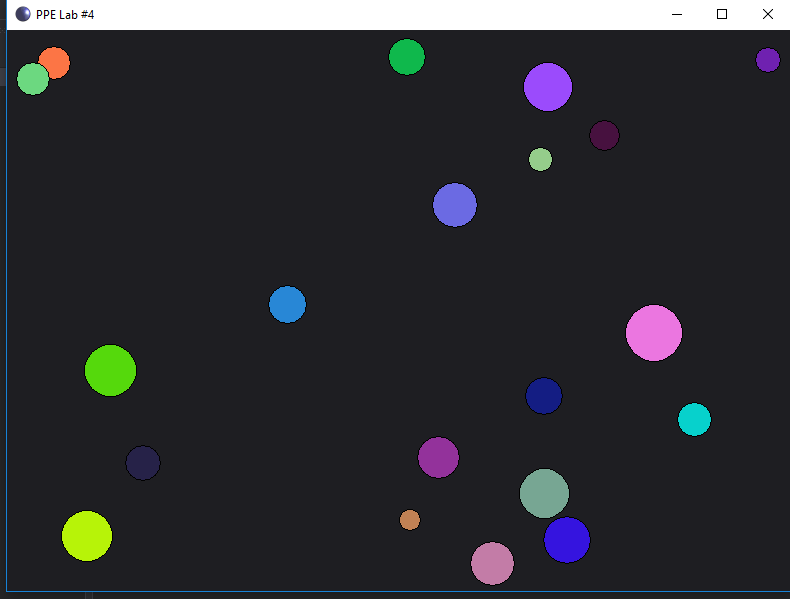
\includegraphics[width=.9\textwidth]{img13.png}
                \caption{The Windows application}
        \end{figure}

\medskip
\newpage
        \subsection*{Conclusion}
        During This lab work i Understand how to add animation in Windows Api. The hardest part was to fix the flickering problem and make realistic behavior of balls during their collision.
\begin{thebibliography}{9}

        \bibitem{sec1}
        Section I, Chapter 8, Programming Windows by Charlez Petzold

\end{thebibliography}
                
\end{document}